\documentclass[10pt,letterpaper]{article}
\usepackage[margin=1in]{geometry}
\usepackage{graphicx}
\usepackage{booktabs}
\usepackage{amsmath}
\usepackage{microtype}
\usepackage[T1]{fontenc}
\usepackage{lmodern}
\usepackage{tikz}
\usetikzlibrary{arrows.meta, positioning, fit, backgrounds}
\usepackage[colorlinks=true, allcolors=blue!60!black]{hyperref}
\usepackage{caption}
\captionsetup{font=small, labelfont=bf}
\usepackage{titlesec}
\titlespacing*{\section}{0pt}{1.5ex plus .3ex}{0.8ex}
\titlespacing*{\subsection}{0pt}{1.2ex plus .3ex}{0.5ex}
\newcommand{\code}[1]{\texttt{\small #1}}

\title{\vspace{-2em}\bfseries mbariml: a curation pipeline for turning deep-sea
imagery and video into object-detection training data}
\author{Lonny Lundsten\\[2pt]
\normalsize Monterey Bay Aquarium Research Institute\\
\normalsize \texttt{lonny@mbari.org}}
\date{\normalsize\today}

\begin{document}
\maketitle

\begin{abstract}
\noindent
Training an object detector for deep-sea ecology is rarely limited by modelling.
It is limited by annotation. A single ROV dive produces hours of footage in which
the animals of interest are sparse, faint, and hard to identify, and every
improvement to the detector requires another round of labelling. \emph{mbariml}
is a pipeline built around that loop rather than around the model. It takes any
Ultralytics YOLO model, runs it over still images or video, stores every
detection as a reviewable region of interest, groups those regions by visual
similarity so that a human can accept or reject them in bulk, and exports the
result as training data. The human review stage is the centre of the design: an
annotator can validate, relabel, resize, delete, and draw entirely new
localizations, and every one of those edits is written back to the same database
the detector wrote to. Video receives particular attention, since an animal held
in frame for three hundred frames should become one training example rather than
three hundred. We describe the pipeline stage by stage, and examine the rule we
use to pick which frame of a track becomes the training crop. That rule rests on
an annotator's judgement that detections are correct more often mid-track. We
find that detector confidence does not follow the same pattern, which suggests
confidence is a poor stand-in for correctness on this footage, and argues for
choosing frames by position rather than by score.
\end{abstract}

\section{The problem}

Consider a typical benthic survey. An ROV flies a transect and records video, or
a camera platform collects stills on a timer. Somewhere in that footage are the
animals an ecologist cares about: sponges, corals, anemones, holothurians, the
occasional fish. They are sparse. They are frequently low-contrast against
sediment. Identifying them to a useful taxonomic level is expert work, and there
is far more footage than expert time.

A detector helps, but not as much as one might hope, and it introduces problems
of its own. Run it at a threshold low enough to catch faint animals and it
returns a large number of false positives that someone must reject. Run it
conservatively and it silently misses the things that most need finding. Either
way the output is a pile of boxes that has to be checked, and checking them one
at a time is no faster than annotating from scratch.

What actually helps is a loop. Over-detect deliberately, group the results so
that hundreds of similar detections can be judged together, let a human correct
what the detector got wrong, and feed the corrected set back into training. The
work in building such a loop is mostly not in the model. It is in keeping the
data in one place, making the human's time count, and getting the result back
out in a form a trainer will accept.

\section{What the pipeline does}

\code{mbariml} is a command-line tool with a graphical review stage, organised
into four phases (Figure~\ref{fig:pipeline}). The sequence is:

\begin{enumerate}\itemsep2pt
\item Point any Ultralytics YOLO model at a folder of images or at video.
\item Get back one row per detection, each carrying its own cropped image.
\item Optionally embed and cluster those crops, then relabel a whole cluster at
      once using its dominant label.
\item Review the result by hand: validate, relabel, adjust boxes, delete
      mistakes, and draw in the detections the model missed.
\item Export training data, summary statistics, or a browsable gallery.
\end{enumerate}

Every one of those steps reads and writes the same DuckDB file, containing a
single flat table in which one row is one region of interest. There is no
per-stage intermediate format. A consequence worth stating plainly: no stage
requires any particular earlier stage to have run, so pointing the video command
at new footage and going straight to review is as valid as running the whole
chain.

\begin{figure}[t]
\centering
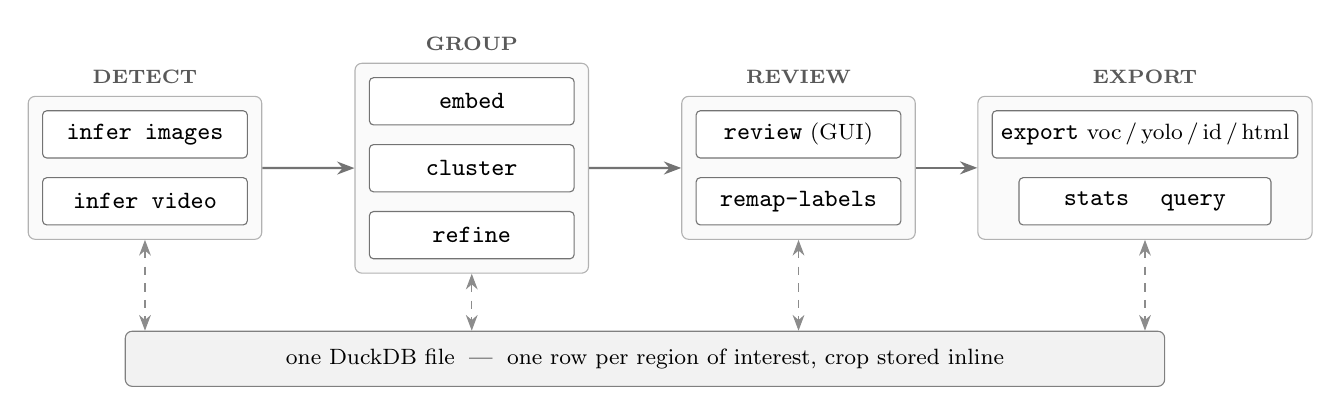
\begin{tikzpicture}[
  box/.style={draw=black!55, rounded corners=1.5pt, align=center, font=\footnotesize,
              minimum height=6mm, minimum width=26mm, inner xsep=3pt, fill=white},
  phase/.style={draw=black!30, rounded corners=2.5pt, inner sep=5pt, fill=black!2},
  lbl/.style={font=\scriptsize\bfseries, black!65},
  ar/.style={-{Stealth[length=2.2mm]}, black!55, thick}]
\node[box] (ii) at (0,0) {\code{infer images}};
\node[box] (iv) at (0,-0.85) {\code{infer video}};
\begin{scope}[on background layer]\node[phase, fit=(ii)(iv)] (p1) {};\end{scope}
\node[lbl, above=1pt of p1] {DETECT};
\node[box] (em) at (4.15,0.42) {\code{embed}};
\node[box] (cl) at (4.15,-0.43) {\code{cluster}};
\node[box] (rf) at (4.15,-1.28) {\code{refine}};
\begin{scope}[on background layer]\node[phase, fit=(em)(cl)(rf)] (p2) {};\end{scope}
\node[lbl, above=1pt of p2] {GROUP};
\node[box] (rv) at (8.3,0) {\code{review} (GUI)};
\node[box] (rm) at (8.3,-0.85) {\code{remap-labels}};
\begin{scope}[on background layer]\node[phase, fit=(rv)(rm)] (p3) {};\end{scope}
\node[lbl, above=1pt of p3] {REVIEW};
\node[box, minimum width=32mm] (ex) at (12.7,0) {\code{export} voc\,/\,yolo\,/\,id\,/\,html};
\node[box, minimum width=32mm] (st) at (12.7,-0.85) {\code{stats} \quad \code{query}};
\begin{scope}[on background layer]\node[phase, fit=(ex)(st)] (p4) {};\end{scope}
\node[lbl, above=1pt of p4] {EXPORT};
\draw[ar] (p1) -- (p2); \draw[ar] (p2) -- (p3); \draw[ar] (p3) -- (p4);
\node[draw=black!50, fill=black!5, rounded corners=2.5pt, font=\footnotesize,
      minimum width=132mm, minimum height=7mm, align=center] (db) at (6.35,-2.85)
      {one DuckDB file \;---\; one row per region of interest, crop stored inline};
\foreach \p in {p1,p2,p3,p4}
  \draw[{Stealth[length=2mm]}-{Stealth[length=2mm]}, black!45, dashed] (\p.south) -- (\p.south |- db.north);
\end{tikzpicture}
\caption{The four phases. All of them read and write the same table, so any
stage's output can be fed to any other stage that needs what it contains.}
\label{fig:pipeline}
\end{figure}

Each row stores its crop inline as a JPEG blob. Embedding, clustering, and the
review mosaic therefore never touch the original imagery, which matters when the
original is a multi-gigabyte video file or a network volume that is not
currently mounted. The full frame is read only when a reviewer wants context or
edits a box.

\section{Detection: any Ultralytics model, stills or video}

The detection stage is a thin layer over
Ultralytics YOLO~\cite{ultralytics}, which does all of the model loading,
inference, and multi-object tracking. Any model Ultralytics can load will work,
including the reader's own fine-tuned weights; nothing in the pipeline is tied to
a particular architecture or class list. Class names are read from the model
itself.

Two presets encode the intent of a run. The \code{curate} preset uses a
confidence threshold of 0.005 and a large inference size, and is meant for
building training data: it over-detects on purpose, because a permissive
threshold can be filtered afterwards while a strict one discards detections that
cannot be recovered without a full re-run. The \code{predict} preset uses 0.08
and is meant for believable inference over new imagery. Both are starting
points rather than fixed values: confidence, IoU, inference size, and the rest
are ordinary options, and passing one overrides whatever the preset would have
supplied.

For each detection the pipeline records the box, the class, the confidence, a
blur score computed from the crop, and the crop itself.

\section{Video: one region of interest per track}

Video needs different treatment from stills. An animal that stays in frame for
three hundred frames produces three hundred detections, and those are not three
hundred training examples. They are one animal, photographed repeatedly. Left
alone they overwhelm clustering, and they make review tedious in a way that
causes annotators to stop paying attention.

The video command therefore runs Ultralytics' tracker and keeps a single region
of interest per track. On a ten-second clip this reduced 711 detections to 7
reviewable observations. The reduction is the point: what reaches the human is a
list of animals, not a list of frames.

Because a track's representative frame cannot be chosen until the track has
finished, this runs as two passes. The first tracks the whole video and retains
only per-track metadata, so memory stays proportional to the number of open
tracks rather than to the length of the video. The second sweeps the file once
and extracts only the chosen frames. That sweep reads forward rather than
seeking: frame-accurate seeking is unreliable on long-GOP encodings, where a
seek lands on the nearest keyframe and would quietly pair a detection's box with
the wrong pixels. A forward sweep is exact, and we verified it by encoding frame
numbers into the pixels of a test video and confirming that the frames returned
carried the numbers requested.

Selected frames are written to disk as ordinary JPEGs, and the row points at the
extracted frame. Video-derived rows are then indistinguishable from
image-derived rows everywhere downstream, so review, embedding, clustering, and
all four exporters work on video without containing any video-specific code. The
link back to the footage is kept in separate columns, which is what lets the
review GUI open the source video at the moment of the detection.

\section{Grouping: embeddings and clusters}

Clustering is optional but changes the economics of review. Each crop is
embedded with DINOv3 (ViT-L/16), and the embeddings are clustered with EVoC.
Each cluster is then labelled with the dominant class among its members, which
propagates one decision across everything in the group. A reviewer looking at a
page of visually similar sponges can accept them together instead of one at a
time.

The same embeddings drive a similarity search in the GUI. Right-clicking any
region of interest re-ranks the entire database by cosine similarity to it,
which turns ``show me the rest of these'' into a single action. Embeddings are
mean-centred on the ranking pool before normalisation; without that step the
component common to nearly all deep-sea imagery dominates the dot product and
compresses similarity into a narrow, weakly separated band.

The search reports the size of the pool it ranked, which is less pedantic than
it sounds. Only regions that already carry an embedding can be ranked, so an
embedding pass that was interrupted or deliberately limited silently reduces
the search to whatever happened to be embedded. The ranked count and the
matching count are displayed together---``all 8,412 matching regions'' against
``3,001 of 8,412''---because the two situations are otherwise indistinguishable
from inside the interface, and the second is easily misread as the search
having covered only the page in view.

Naming the clusters turns out to need care. The obvious approach, and the one
we started with, is to label a cluster after the dominant original class among
its members. That assumes the detector has enough classes for the label to
distinguish one cluster from another, which is not always true. A single-class
detector---MBARI's Megalodon, for instance, which reports only \code{object}---
makes every cluster's dominant label the same string, so writing it back
collapses the clustering that was just computed into one undifferentiated
label. The structure survives only in the raw cluster number, and the review
GUI, which filters and sorts on the curated label, can no longer separate the
groups at all.

Clusters are therefore named with an index appended whenever one label wins
more than one cluster: a single-class run yields \code{object\_1},
\code{object\_2}, and so on. On a 147-region run from a single-class model,
six clusters that previously all became \code{object} now come back separately
labelled. The same rule helps multi-class runs, where several clusters of the
same taxon would otherwise be flattened together; on the same regions with the
detector's real labels, two singleton clusters keep their bare names while four
distinct sponge clusters become \code{Hexactinellida\_1} through
\code{\_4}. Merging them afterwards is one bulk relabelling command, whereas
recovering a distinction that was thrown away is not.

Which label the naming vote reads is itself a choice, and defaulting it to the
detector's raw class is wrong as soon as a database has been reviewed. The
human decisions live in the curated label, and on a single-class model the raw
class is the same useless string for every region, so re-clustering a reviewed
database discarded the review twice over: the write-back replaces the curated
label, and the replacement was voted on from a column the reviewer never
touched. The naming vote can now be pointed at the curated label instead,
falling back to the raw class for regions not yet reviewed. On a 300-region
database curated into three taxa, the default returns three indexed
\code{object} names while the curated source returns the three taxon names.

This is worth stating alongside a caveat the command cannot enforce: the
write-back replaces the curated label for every embedded region, including ones
already marked verified, and does not clear the verified flag---so those rows
afterwards appear reviewed while carrying a machine-generated name. Clustering
experiments therefore belong on a copy of the database. The copy carries the
embeddings, so the expensive stage is not repeated and each iteration costs
seconds.

When the first clustering pass lumps things too coarsely, a refine step
re-clusters a single label into finer groups, which is the usual remedy for a
large catch-all bucket.

\section{Review: the human in the loop}

Everything above exists to make this stage efficient. The detector proposes; the
annotator decides. The review GUI (Figure~\ref{fig:gui}) presents regions of
interest as a mosaic of crops, tinted by label, with a badge marking those that
have been checked. An annotator working through a page can:

\begin{itemize}\itemsep1.5pt
\item \textbf{Validate} a detection, marking it reviewed. Applying a label counts
      as review, since labelling something is itself an act of checking it.
\item \textbf{Relabel} one region or a selection of hundreds, either by typing a
      new concept or picking one already in use in this database.
\item \textbf{Adjust} a box by dragging its handles on the full-resolution frame.
      The stored crop is regenerated to match, immediately.
\item \textbf{Delete} false positives, individually or in bulk.
\item \textbf{Add} a localization the model missed entirely, by drawing a box on
      the frame and naming it. Its embedding is computed in the background using
      the same model and preprocessing as the batch path, so a hand-drawn region
      is directly comparable to every other one and participates in similarity
      search straight away.
\end{itemize}

\begin{figure}[t]
\centering
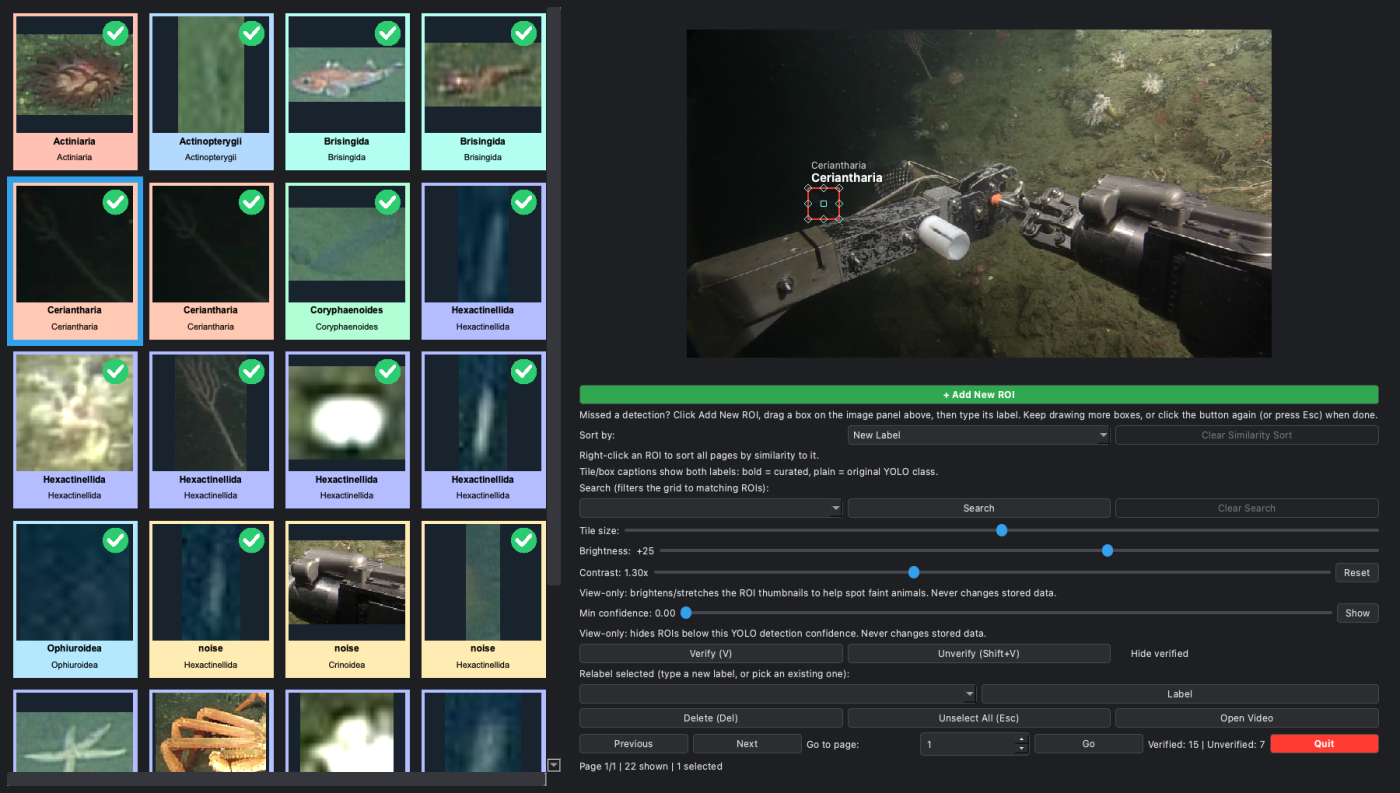
\includegraphics[width=\textwidth]{../review_gui.png}
\caption{The review GUI. Left: the mosaic of regions of interest, tinted by
label, with a badge on those already checked. Right: the full source frame with
every detection on it drawn as an editable box, above the controls. Brightness
and contrast sliders stretch the thumbnails without altering stored data, which
matters for faint animals against sediment. ``Open Video'' is active here
because this region came from video, and opens the footage at the moment of the
detection.}
\label{fig:gui}
\end{figure}

Two details turned out to matter more than expected. The first is that the
right-hand panel draws \emph{every} detection on the source frame, not only the
ones on the current page, because detections from the same frame are often
scattered across different pages by sorting. Without this, a reviewer editing a
box has no idea what else was found on that image. The second is a pair of
brightness and contrast sliders. Deep-sea imagery is frequently dark and
low-contrast, and animals that are invisible at native exposure become obvious
when stretched. The adjustment applies to the displayed thumbnails only and
never modifies stored data.

A separate bulk relabelling command handles taxonomy revisions across an entire
database, applying all renames in a single pass so that a file which swaps two
labels does what it says.

\section{Choosing which frame represents a track}

Reducing a track to one region raises the obvious question of which frame to
keep. Our default takes the highest-confidence detection from the middle third
of the track.

The reasoning comes from reviewing this kind of footage. An animal enters the
field of view at the edge of the frame, passes through the region where the
camera is best focused and best positioned, and then leaves. Detections made
during that middle interval are, in our annotators' experience, \emph{correct}
more often: the identification survives expert review more frequently than one
made as the animal entered or left. Figure~\ref{fig:track}(a,b) shows a track
that behaves this way, with the crops from mid-transit better framed and
sharper than those at either end.

That claim is about correctness as judged by a person, which is not the same
quantity as the detector's own confidence score. The difference is worth
keeping in view, because the two can disagree: a model can be confidently wrong
about a poorly framed animal, and unsure about a well-framed one it happens to
have seen rarely in training.

We measured the confidence side across 19 tracks from three clips, and it does
\emph{not} show a middle-third peak. Confidence is highest in the first third
for 9 of the 19 tracks, in the middle third for 4, and in the last third for 6,
and the middle third has the lowest mean of the three (0.301, against 0.333 for
the first third; Figure~\ref{fig:track}(c)). Some of this is geometry: an ROV
often approaches an animal and stops, or passes close enough that the view keeps
improving until the track ends, so the best frames are the last ones rather than
the middle ones. Two of the longest tracks we examined behave that way.

\begin{figure}[t]
\centering
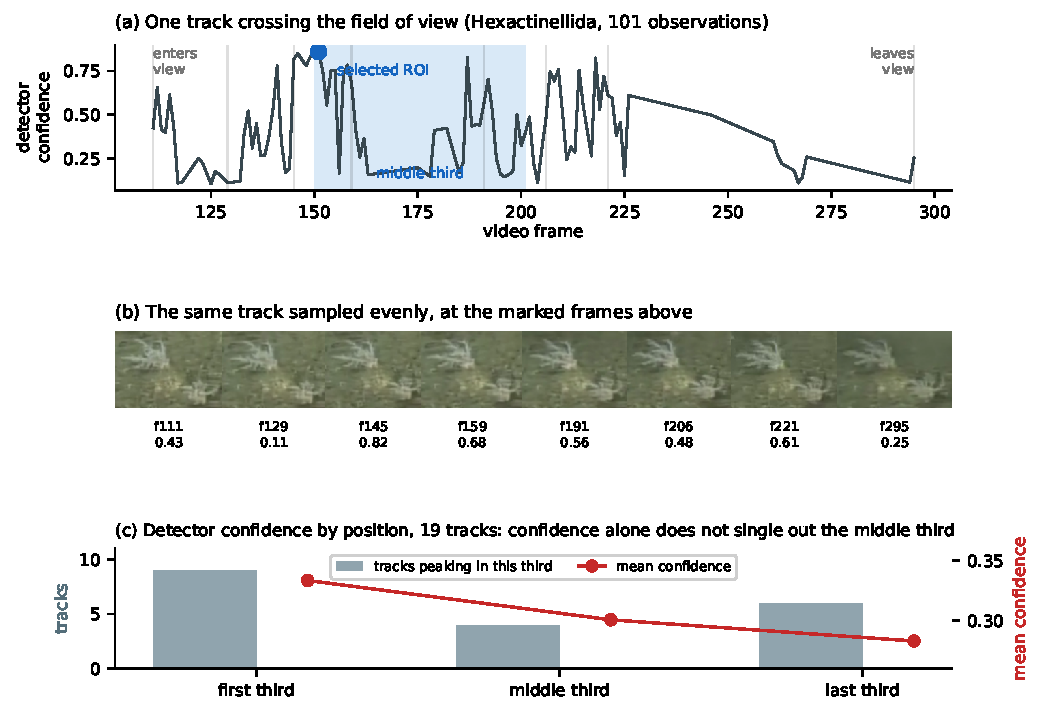
\includegraphics[width=0.98\textwidth]{fig/track_selection.pdf}
\caption{Choosing a frame from a track. (a) Detector confidence across one
101-observation track, with the middle third shaded and the selected region
marked. (b) The same track sampled evenly at the frames marked in (a); the
animal is best framed part-way through the transit. (c) Detector confidence
across 19 tracks from three clips does not single out the middle third: it peaks
in the first third more often than in the middle, and the middle third has the
lowest mean. Confidence is a different quantity from the human-assessed
correctness the rule is based on.}
\label{fig:track}
\end{figure}

The two observations are not in conflict, and the disagreement is the
interesting part. If human-assessed correctness does peak mid-track while
confidence does not, then confidence is not tracking correctness on this
footage, and picking a frame by score alone would be the wrong thing to do. A
positional rule is then doing work that a confidence threshold cannot.

We have not closed the loop on this. Establishing the correctness claim properly
means reviewing detections sampled from the first, middle, and last thirds of
many tracks and recording how often each is right, which is expert time we have
not yet spent. Until then the middle-third rule stands as an informed default
rather than a measured one, and the alternatives---highest confidence anywhere
in the track, the sharpest frame in the middle third, or the exact centre
frame---are selectable per run.

\section{Getting the data back out}

The export stage writes Pascal VOC XML, YOLO-format label files with the
accompanying names file, \code{*.id} sidecar files placed beside the source
images for MBARI's own tooling, and a paginated HTML gallery for quick visual
checks. The VOC and YOLO exports also emit a manifest of the source images and a
small standalone script that copies them, since annotation files are of no use
to a trainer without the imagery beside them.

The YOLO export additionally writes the train, validation and test image lists,
which completes the dataset rather than leaving the last step to be done by
hand. Two decisions in how they are written are worth recording. The listed
paths are relative to the dataset directory, so the directory refers only to
itself and can be archived or moved to a training machine without any path
being rewritten---absolute paths recorded on the exporting machine could not
survive that move. And the split is taken over images, never over individual
detections. Two crops of the same frame placed on opposite sides of the
train/validation boundary share their background, their illumination and often
the same individual animal, which inflates validation scores on transect
imagery where consecutive frames already overlap heavily. The split is seeded
by default for the same reason the rest of the pipeline is reproducible: a
re-export after correcting a handful of labels should not quietly reshuffle
which images were held out, since that would make models trained either side
of the re-export incomparable.

Two commands support analysis rather than training. A statistics command reports
label counts and per-image detection counts, and writes a label-by-image matrix
suitable for ecological work such as per-image richness or frequency of
occurrence. An ad hoc query command runs arbitrary SQL against the database,
which is often the fastest way to answer a question the tool does not
anticipate.

\section{Limitations}

The evaluation here is internal and small. We report data-reduction and
throughput figures, not detection accuracy. The track-selection rule in
particular rests on an annotator's judgement that has not been quantified: the
experiment that would settle it is a review pass over detections sampled from
each third of many tracks, scoring how often each is correct, followed by
training runs on datasets built under each rule. The longest video
processed end to end is short; the first pass retains only metadata and should
scale flatly with duration, but this is unverified at full dive length.
Clustering quality depends on EVoC parameters that in practice need tuning per
deployment. Because DuckDB takes an exclusive lock on the database file, two
people cannot curate the same database at once, and combining separately curated
databases is a manual merge.

\section{Availability and credits}

\code{mbariml} is written in Python and available at
\url{https://github.com/mbari-org/mbari-ml}.

Detection and tracking are provided entirely by \textbf{Ultralytics
YOLO}~\cite{ultralytics}, which the pipeline wraps rather than reimplements;
model loading, inference, and the multi-object trackers are all theirs. The
review GUI's mosaic rendering, threading, and box-overlay machinery are adapted
from MBARI's \emph{vars-gridview}~\cite{varsgridview} under the MIT licence.
Embeddings use DINOv3~\cite{dinov3} via \code{timm}, clustering uses
EVoC~\cite{evoc}, and storage is DuckDB~\cite{duckdb}. The database layer, the
video ingest and track-reduction stages, the export formats, and the additions
to the review GUI described here are original to this work.

\begin{thebibliography}{9}\small
\bibitem{ultralytics} G. Jocher, J. Qiu, and A. Chaurasia. \emph{Ultralytics
YOLO}. \url{https://github.com/ultralytics/ultralytics}, 2023--.
\bibitem{varsgridview} Monterey Bay Aquarium Research Institute.
\emph{vars-gridview}. \url{https://github.com/mbari-org/vars-gridview}.
\bibitem{dinov3} Meta AI Research. \emph{DINOv3: self-supervised vision
transformers}, 2025.
\bibitem{evoc} L. McInnes. \emph{EVoC: embedding vector oriented clustering}.
\url{https://github.com/TutteInstitute/evoc}.
\bibitem{duckdb} M. Raasveldt and H. M\"uhleisen. DuckDB: an embeddable
analytical database. In \emph{SIGMOD}, 2019.
\end{thebibliography}

\end{document}
